\chapter*{Introduction} \label{intro:chapter}
%mbxSTARTIGNORE
\addfakecontentsline{Introduction}
\markboth{INTRODUCTION}{INTRODUCTION}
%mbxENDIGNORE

%%%%%%%%%%%%%%%%%%%%%%%%%%%%%%%%%%%%%%%%%%%%%%%%%%%%%%%%%%%%%%%%%%%%%%%%%%%%%%

\section{Notes \`a propos de ce manuel}
\label{notes:section}

%\sectionnotes{\`A propos de l'auteur.}
Ceci est une traduction d'un manuel libre écrit par Ji\v{r}i Lebl.  Il s'agit d'un premier cours d'équations diff\'erentielles pour les personnes \'etudiant en g\'enie.

Originalement des notes pour
un cours enseign\'e 
\`a \href{https://www.math.uiuc.edu/}{University of Illinois at
Urbana-Champaign} en 2008-2009, l'auteur  les a utilisées ensuite 
\`a UIUC\@, \href{https://www.math.ucsd.edu/}{University of California, San Diego} (UCSD),
et \href{https://math.okstate.edu/}{Oklahoma State University} (OSU).
Normalement, ces cours sont enseign\'es avec le manuel de 
Edwards and Penney, \emph{Differential
Equations and Boundary Value Problems: Computing and Modeling}~\cite{EP}, ou de Boyce et DiPrima,
\emph{Elementary
Differential Equations and Boundary Value Problems}~\cite{BD},
et ce livre-ci se veut un remplacement de ces ressources.

L'adaptation en français a été écrite pour les cours de GCH217 et MAT217 donnés à l'Université de Sherbrooke.

Voici d'autres références :
E.L.\ Ince,
\emph{Ordinary Differential Equations}~\cite{I}, classique (et \'economique);
Stanley Farlow, \emph{Differential Equations and Their
Applications}~\cite{F}; 
Berg and McGregor,
\emph{Elementary Partial Differential Equations}~\cite{BM}, maintenant disponible dans Dover;
et William Trench,
\emph{Elementary
Differential Equations with Boundary Value Problems}~\cite{T}, ressource libre.
Voir le chapitre \hyperref[furtherreading:chapter]{Lectures additionnelles} \`a la fin de ce livre.

%\subsection{Organisation}
%
%L'organisation de ce livre requiert que les chapitres soient abord\'es dans l'ordre.  Les chapitres de la fin peuvent \^etre omis.  L'interd\'ependance du contenu est comme suit.
%
%% If changing make sure to also update figures/chapterdiagram.pdf_t
%% That's a hopefully short term hack before I figure out how to do it
%% better so that it also gets links and such
%%mbxSTARTIGNORE
%
%\begin{equation*}
%\begin{tikzcd}[cramped, row sep=small]
%& {\text{\hyperref[intro:chapter]{Introduction}}} \arrow[d] \\
%{\text{\Appendixref{linalg:appendix}}} \arrow[dd, dotted]
%& {\text{\Chapterref{fo:chapter}}} \arrow[d] \\
%& {\text{\Chapterref{ho:chapter}}} \arrow[dddr] \arrow[dd] \arrow[dl] \arrow[dr] \\
%{\text{\Chapterref{sys:chapter}}} \arrow[dr, dotted] \arrow[d] & 
%  {\text{\Chapterref{ps:chapter}}} \\
%{\text{\Chapterref{nlin:chapter}}} & {\text{\Chapterref{FS:chapter}}} \arrow[d]
%\arrow[dr,dotted] \\
%& {\text{\Chapterref{SL:chapter}}}
%& {\text{\Chapterref{LT:chapter}}}
%\end{tikzcd}
%\end{equation*}
%
%%mbxENDIGNORE
%%mbxlatex \begin{center}
%%mbxlatex \inputpdft{chapterdiagram}
%%mbxlatex \end{center}
%
%Les chapitres \ref{FS:chapter} et \ref{SL:chapter} contiennent certaines r\'ef\'erences au
% \chapterref{sys:chapter} (un peu d'alg\`ebre lin\'eaire), mais ces r\'ef\'erences ne sont pas essentielles et peuvent \^etre parcourues rapidement.
%Quant au \chapterref{LT:chapter}, il ne d\'epend pas de \chapterref{FS:chapter} sauf pour la section sur les EDP \ref{laplacepde:section},
%Cependant, en th\'eorie il pourrait \^etre couvert de mani\`ere ind\'ependante.
%L'\appendixref{linalg:appendix} couvre de mani\`ere plus substantielle l'alg\`ebre lin\'eaire que la section de r\'evision
% \sectionref{sec:matrix}, pour un cours combinant l'alg\`ebre lin\'eaire et les \'equations diff\'erentielles ordinaires\@.

%\medskip
%\subsection{Typical types of courses}
%
%Several typical types of courses can be run with the book.
%There are the two original courses at UIUC\@,
%both cover ODE as well some PDE\@.
%Either, there is the 4 hours-a-week for a semester (Math 286 at UIUC):
%
%\medskip
%
%\noindent
%\hyperref[intro:chapter]{Introduction} (\ref{introde:section}),
%\chapterref{fo:chapter} (\ref{integralsols:section}--\ref{numer:section}),
%\chapterref{ho:chapter},
%\chapterref{sys:chapter},
%\chapterref{FS:chapter} (\ref{bvp:section}--\ref{dirich:section}),
%\chapterref{SL:chapter} (or
%\ref{LT:chapter} or \ref{ps:chapter} or \ref{nlin:chapter}).
%
%\medskip
%
%Or, the second course at UIUC is at 3 hours-a-week (Math 285 at UIUC):
%
%\medskip
%
%\noindent
%\hyperref[intro:chapter]{Introduction} (\ref{introde:section}),
%\chapterref{fo:chapter} (\ref{integralsols:section}--\ref{numer:section}),
%\chapterref{ho:chapter},
%\chapterref{FS:chapter} (\ref{bvp:section}--\ref{dirich:section}),
%(and maybe \chapterref{SL:chapter},
%\ref{LT:chapter}, or \ref{ps:chapter}).
%
%\medskip
%
%A semester-long course at 3 hours a week that doesn't cover either systems or PDE
%will cover, beyond the introduction,
%%\sectionref{introde:section},
%\chapterref{fo:chapter},
%\chapterref{ho:chapter},
%\chapterref{LT:chapter}, and \chapterref{ps:chapter},
%(with sections skipped as above).
%On the other hand, a typical course that covers 
%systems will probably need to skip Laplace and power series
%and cover
%%\sectionref{introde:section},
%\chapterref{fo:chapter},
%\chapterref{ho:chapter},
%\chapterref{sys:chapter}, and \chapterref{nlin:chapter}.
%
%\medskip
%
%If sections need to be skipped in the beginning, a good core of the 
%sections on single ODE is:
%\ref{introde:section},
%\ref{integralsols:section}--\ref{intfactor:section},
%\ref{auteq:section},
%\ref{solinear:section},
%\ref{sec:ccsol},
%\ref{sec:mv}--\ref{forcedo:section}.
%
%\medskip
%
%The complete book can be covered at a reasonably
%fast pace at approximately 76 lectures
%(without \appendixref{linalg:appendix})
%or 86 lectures (with \appendixref{linalg:appendix} replacing
%\sectionref{sec:matrix}).
%This is not accounting for exams, review,
%or time spent in a computer lab. % (if using IODE for example).
%A two-quarter or a two-semester course can be easily run with the material.
%For example (with some sections perhaps strategically skipped):
%
%\medskip
%
%\noindent
%Semester 1:
%\hyperref[intro:chapter]{Introduction},
%\chapterref{fo:chapter},
%\chapterref{ho:chapter},
%\chapterref{LT:chapter},
%\chapterref{ps:chapter}.
%\\
%Semester 2: 
%\Chapterref{sys:chapter},
%\chapterref{nlin:chapter},
%\chapterref{FS:chapter},
%\chapterref{SL:chapter}.
%
%\medskip
%
%A combined course on ODE with linear algebra can run as:
%
%\medskip
%
%\noindent
%\hyperref[intro:chapter]{Introduction},
%\chapterref{fo:chapter} (\ref{integralsols:section}--\ref{numer:section}),
%\chapterref{ho:chapter},
%\appendixref{linalg:appendix},
%\chapterref{sys:chapter} (w/o \sectionref{sec:matrix}), (possibly 
%\chapterref{nlin:chapter}).
%
%\medskip
%
%The chapter on
%the Laplace transform (\chapterref{LT:chapter}),
%the chapter on Sturm--Liouville (\chapterref{SL:chapter}),
%the chapter on power series (\chapterref{ps:chapter}),
%and the chapter on nonlinear systems (\chapterref{nlin:chapter}),
%are more or less interchangeable and can be treated as \myquote{topics}.
%If \chapterref{nlin:chapter} is covered, it may be best to place it right 
%after \chapterref{sys:chapter},
%and \chapterref{SL:chapter} is best covered right after
%\chapterref{FS:chapter}.
%If time is short, the first two sections of
%\chapterref{ps:chapter} make a reasonable self-contained unit.

%%\medskip
%\subsection{Computer resources}
%
%The book's
%website \url{https://www.jirka.org/diffyqs/}
%contains the following resources:
%\begin{enumerate}
%\item Interactive SAGE demos.
%\item Online WeBWorK homeworks
%(using either your own WeBWorK installation or Edfinity)
%for most sections, customized for this book.
%\item The PDFs of the figures used in this book.
%\end{enumerate}
%
%I taught the UIUC courses using IODE\index{IODE software}
%(\url{https://faculty.math.illinois.edu/iode/}).
%IODE is a free software package that
%works with Matlab (proprietary) or Octave (free software).
%%Unfortunately IODE is not kept up to date at this point, and may have
%%trouble running on newer versions of Matlab.
%The graphs in the book were made with
%the Genius\index{Genius software} software
%(see \url{https://www.jirka.org/genius.html}).  I use Genius
%in class to show these (and other) graphs.
%
%The \LaTeX\ source of the book is also available
%for possible modification and customization
%at github (\url{https://github.com/jirilebl/diffyqs}).
%
%%\medskip
%
%%\textbf{Acknowlegements:}
%
%\subsection{Acknowledgments}
%
%Firstly, I would like to acknowledge Rick Laugesen.  I used his handwritten
%class notes
%the first time I taught
%Math 286.  My organization of this book through chapter 5,
%and the choice of
%material covered, is heavily influenced by his notes.  Many
%examples and computations are taken from his notes.  I am also heavily
%indebted to Rick for all the advice he has given me, not just on teaching
%Math 286.
%For spotting errors and other suggestions,
%I would also like to acknowledge (in no particular order):
%John P.\ D'Angelo,
%Sean Raleigh, Jessica Robinson, Michael Angelini, Leonardo Gomes, Jeff
%Winegar, Ian Simon, Thomas Wicklund, Eliot Brenner, Sean Robinson,
%Jannett Susberry, Dana Al-Quadi, Cesar Alvarez, Cem Bagdatlioglu,
%Nathan Wong, Alison Shive, Shawn White, Wing Yip Ho, Joanne Shin,
%Gladys Cruz, Jonathan Gomez, Janelle Louie, Navid Froutan,
%Grace Victorine, Paul Pearson, Jared Teague, Ziad Adwan,
%Martin Weilandt, S\"{o}nmez \c{S}ahuto\u{g}lu,
%Pete Peterson, Thomas Gresham, Prentiss Hyde, Jai Welch,
%Simon Tse, Andrew Browning, James Choi, Dusty Grundmeier,
%John Marriott,
%Jim Kruidenier,
%Barry Conrad,
%Wesley Snider,
%Colton Koop,
%Sarah Morse,
%Erik Boczko,
%Asif Shakeel,
%Chris Peterson,
%Nicholas Hu,
%Paul Seeburger,
%Jonathan McCormick,
%David Leep,
%William Meisel,
%Shishir Agrawal,
%Tom Wan,
%Andres Valloud,
%and probably others I
%have forgotten.
%Finally, I would like
%to acknowledge NSF grants DMS-0900885 and DMS-1362337.
%

%%%%%%%%%%%%%%%%%%%%%%%%%%%%%%%%%%%%%%%%%%%%%%%%%%%%%%%%%%%%%%%%%%%%%%%%%%%%%%

\sectionnewpage
\section{Introduction aux \'equations diff\'erentielles}
\label{introde:section}

%\sectionnotes{more than 1 lecture\EPref{, \S1.1 in \cite{EP}}\BDref{,chapter 1 in \cite{BD}}}

\subsection{\'Equations diff\'erentielles}

Les lois de la physique sont g\'en\'eralement exprim\'ees sous forme d'\'equations diff\'erentielles.  Ainsi, toute discipline de science ou de g\'enie utilise les \'equations diff\'erentielles, \`a un niveau plus ou moins sophistiqu\'e.  Comprendre les \'equations diff\'erentielles est essentiel \`a la compr\'ehension de presque tout ce que vous apprendrez dans vos classes de science ou de g\'enie.  On peut penser aux math\'ematiques comme le langage de la science, et les \'equations diff\'erentielles forment une partie importante de ce langage.
%As an analogy,
%suppose all your classes from now on were given in Swahili.  
%It would be important to first learn Swahili, or you would have a very
%tough time getting a good grade in your classes.

Vous avez d\'ej\`a vu plusieurs \'equations diff\'erentielles, peut-\^etre sans savoir que c'en \'etait.
Et vous avez m\^eme r\'esolu des \'equations diff\'erentielles dans vos cours de calcul.  Voyons un exemple que vous n'avez peut-\^etre pas vu:
\begin{equation} \label{eq1}
\frac{dx}{dt} + x = 2 \cos t .
\end{equation}
Ici $x$ est la  \emph{\myindex{variable d\'ependante}} et $t$ est la \emph{\myindex{variable ind\'ependante}}.
L'équation \eqref{eq1}
est un exemple de base d'une \emph{\myindex{\'equation diff\'erentielle}}. Plus pre\'cis\'ement, c'est un exemple d'\emph{\myindex{\'equation diff\'erentielle du premier ordre}}, puisqu'elle n'implique que la premi\`ere d\'eriv\'ee de la variable d\'ependante $x$.  Cette \'equation vient de la loi du refroidissement de Newton, lorsque la temp\'erature ambiante oscille en fonction du temps.

\subsection{Solutions d'\'equations diff\'erentielles}

Quand on résoud une \'equation diff\'erentielle comme \eqref{eq1}, l'inconnue est une variable $x$, qui elle-même d\'epend d'une variable $t$.  C'est-\`a-dire, on veut trouver un $x$, dépendant de $t$, tel que, lorsqu'on substitue $x$, $t$ et $\frac{dx}{dt}$ dans l'équation \eqref{eq1}, le c\^ot\'e gauche est \'egal au c\^ot\'e droit et donc l'\'egalit\'e est satisfaite.  C'est le m\^eme principe que pour une \'equation ordinaire (alg\'ebrique) impliquant $x$ et $t$.  Nous affirmons que l'expression suivante est une \emph{\myindex{solution}}\,: 
\begin{equation*}
x = x(t) = \cos t + \sin t .
\end{equation*}
%
Comment le v\'erifier?  Il suffit de substituer $x$ dans l'\'equation \eqref{eq1} et vérifier que l'égalité est bel et bien établie.    Nous devons d'abord calculer $\frac{dx}{dt}$.  On trouve que $\frac{dx}{dt} = 
-\sin t + \cos t$.  Maintenant, calculons le c\^ot\'e gauche de \eqref{eq1}\,: 
\begin{equation*}
\frac{dx}{dt} + x = 
\underbrace{(-\sin t + \cos t)}_{\frac{dx}{dt}}
+
\underbrace{(\cos t + \sin t)}_{x}
=
2\cos t .
\end{equation*}
C'est bien ce qu'on veut\,: nous obtenons exactement le c\^ot\'e droit de l'\'equation.
Mais ce n'est pas tout. 
Nous affirmons que 
$x = \cos t + \sin t + e^{-t}$ est aussi une solution.  Vérifions\,: 
\begin{equation*}
\frac{dx}{dt} = -\sin t + \cos t - e^{-t} .
\end{equation*}
On remplace ceci dans \eqref{eq1}\,: 
\begin{equation*}
\frac{dx}{dt} + x = 
\underbrace{(-\sin t + \cos t - e^{-t})}_{\frac{dx}{dt}} +
\underbrace{(\cos t + \sin t + e^{-t})}_{x}
= 2\cos t .
\end{equation*}
Il s'agit bien d'une solution.

Ainsi, plusieurs solutions sont possibles.  Pour cette \'equation en particulier, toutes les solutions peuvent s'\'ecrire sous la forme\,; 
\begin{equation*}
x = \cos t + \sin t + C e^{-t} 
\end{equation*}
pour une constante $C$.  Diff\'erentes constantes $C$ donneront des solutions diff\'erentes, donc il y a vraiment un nombre infini de solutions possibles.  Voir la~\figurevref{intro:plotsfig} pour le graphe de quelques solutions.  Nous verrons un peu plus tard comment trouver ces solutions de mani\`ere g\'en\'erale.

\medskip

\begin{mywrapfig}{3.25in}
\capstart
\diffyincludegraphics{width=3in}{width=4.5in}{intro-plots-alt}
\caption{Quelques solutions de $\frac{dx}{dt} + x = 2 \cos t$.\label{intro:plotsfig}}
\end{mywrapfig}%

La résolution d'une \'equation diff\'erentielle peut \^etre tr\`es ardue.  Il n'y a pas une m\'ethode g\'en\'erale pour les r\'esoudre toutes. La plupart du temps, nous verrons comment obtenir des formules exactes pour r\'esoudre certaines \'equations diff\'erentielles, mais parfois nous n'obtiendrons que des solutions approximatives,  De plus, nous passerons un peu de temps \`a comprendre certaines \'equations, sans les r\'esoudre.

La majeure partie de ce livre est d\'edi\'ee aux 
\emph{\'equations diff\'erentielles ordinaires\index{ordinary differential equation}}
ou EDO\index{ODE}, c'est-\`a-dire des \'equations ayant une seule variable ind\'ependante, o\`u les d\'eriv\'ees se prennent en termes de cette unique variable.  Lorsqu'il y a plusieurs variables ind\'ependantes, on obtient des 
\emph{\'equations aux d\'eriv\'ees partielles \index{partial differential equation}}
ou EDP\index{PDE}.
%We will briefly see these near the
%end of the course.

M\^eme pour les EDO, qui sont tr\`es bien comprises, il ne s'agit pas simplement de tourner une manivelle pour obtenir une r\'eponse.  
%When you can find exact solutions, they are usually preferable to approximate solutions.  
  C'est important de comprendre comment de telles solutions sont trouv\'ees.  M\^eme si, dans la vraie vie, vous laisserez la plupart des calculs \`a des ordinateurs, vous devez comprendre ce qu'ils font.  Il est parfois n\'ecessaire de simplifier ou transformer votre \'equation pour que la machine la comprenne et la r\'esoude.  Il vous faudra peut-\^etre m\^eme ajouter ou modifier des hypoth\`eses dans votre mod\`ele pour ce faire.
  
Pour r\'eussir en g\'enie ou en sciences, vous aurez \`a r\'esoudre des probl\`emes dans votre travail que vous n'aurez jamais vus auparavant.  D'o\`u l'importance d'apprendre des techniques de r\'esolution de probl\`emes, afin d'appliquer ces techniques aux nouveaux probl\`emes.  
%Une erreur courante est de s'attendre \`a une recette qui r\'soudre tous les probl\`emes que vous rencontrerez.  Ce cours n'est pas une exception.
 
\subsection{En pratique}
\begin{myfig}
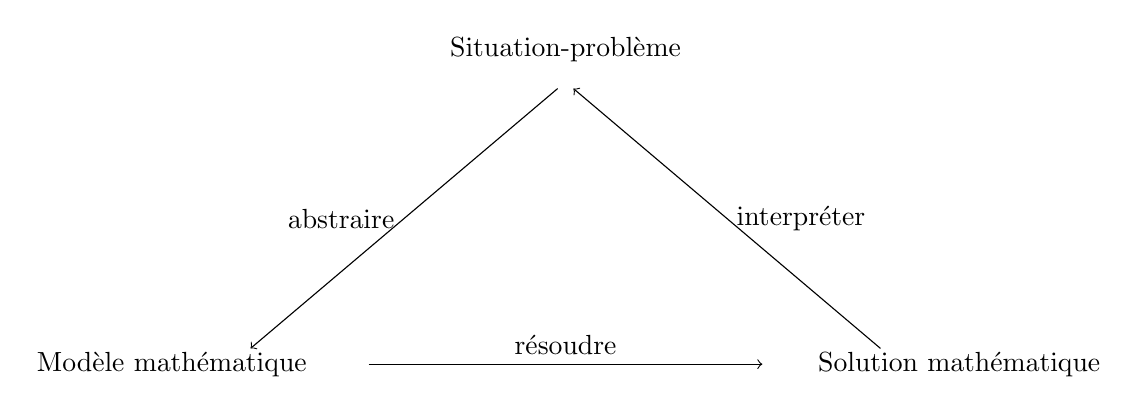
\begin{tikzpicture}
\draw (0,0) node {Situation-problème};
\draw[->] (-0.1,-0.5) -- (-4,-3.8) node[left,pos=0.5] {abstraire};
\draw (-5,-4) node {Modèle mathématique} ;
 \draw[->]
(-2.5,-4) -- (2.5,-4) node [above, pos=0.5] {résoudre};
\draw (5,-4)  node {Solution mathématique};
\draw[->] (4,-3.8) -- (0.1,-0.5)  node[right,pos=0.5] {interpréter};
\end{tikzpicture}
\end{myfig}

%\begin{mywrapfigsimp}{3.05in}{3.35in}
%\noindent
%\inputpdft{1-1-fig}
%\diffypdfversion{\par\vspace*{5pt}}
%\end{mywrapfigsimp}
Comment utilise-t-on les \'equations diff\'erentielles en sciences et en g\'enie?  On commence avec une \emph{\myindex{situation-probl\`eme}} qu'on veut comprendre.  \`A l'aide d'hypoth\`eses suppl\'ementaires pour simplifier le probl\`eme, on cr\'ee un 
\emph{\myindex{mod\`ele math\'ematique}}.  Autrement dit, on traduit la situation en \'equations diff\'erentielles.  Ensuite, on utilise les math\'ematiques afin d'obtenir une \emph{\myindex{solution math\'ematique}}.  Mais ce n'est pas fini.  Il faut encore interpr\'eter les r\'esultats\,: qu'est-ce que la solution math\'ematique nous dit \`a propos de la situation-probl\`eme de d\'epart?

Pour ce qui est de formuler le mod\`ele math\'ematique, et d'interpr\'eter les r\'esultats, vous ferez cela surtout dans vos cours de g\'enie et de sciences.  Dans ce cours-ci, nous nous concentrerons principalement sur l'analyse math\'ematique.  Parfois, nous travaillerons avec des exemples r\'ealistes simples, afin de d\'evelopper notre intuition et motiver les concepts que nous verrons.

Consid\'erons ici un exemple.  Une des \'equations les plus fondamentales est le \emph{\myindex{mod\`ele de croissance exponentielle}}.  D\'enotons une population de bact\'eries par la variable $P$ (plus pr\'ecis\'ement, $P$ d\'enote la quantit\'e de population).  On suppose que l'environnement contient suffisamment de nutriments et d'espace.  Dans ce cas-l\`a, le taux de croissance de la population de bact\'eries est proportionnelle \`a la population -- une population plus nombreuse cro\^itra plus rapidement.  D\'enotons le temps (en secondes, disons) par la variable $t$.  Notre mod\`ele est alors\,: 
%
\begin{equation*}
\frac{dP}{dt} = kP 
\end{equation*}
o\`u $k > 0$ est une constante.

\begin{example}
Supposons qu'il y a 100 bact\'eries au temps 0 et 200 bact\'eries 10 secondes plus tard.  Combien aura-t-on de bact\'eries \`a une minute (60 secondes) du d\'ebut?

%mbxSTARTIGNORE
%mbxENDIGNORE
%
% Make sure to keep the above and the mbx figure below in sync!
%
D'abord, nous devons r\'esoudre l'\'equation diff\'erentielle.  Nous affirmons que la fonction suivante est une solution\,: 
\begin{equation*}
P(t) = C e^{kt} 
\end{equation*}
o\`u $C$ est une constante.  V\'erifions ceci\,: 
\begin{equation*}
\frac{dP}{dt} = C k e^{kt} = k P .
\end{equation*}
Il s'agit donc bel et bien d'une solution.

Ensuite?  On ne connait pas la valeur de $C$, ni de $k$.  Mais on sait ceci.
On sait que $P(0) = 100$, et on sait que
$P(10) = 200$.  Substituons ces valeurs dans l'expression et regardons ce qu'on obtient\,: 
\begin{align*}
& 100 = P(0) = C e^{k0} = C ,\\
& 200 = P(10) = 100 \, e^{k10} .
\end{align*}
Par cons\'equent, $2 = e^{10k}$ ou $\frac{\ln 2}{10} = k \approx 0.069$.
Donc\,: 
\begin{equation*}
P(t) = 100 \, e^{(\ln 2) t / 10} \approx 100 \, e^{0.069 t} .
\end{equation*}
\`A une minute, $t=60$, la population est $P(60) = 6400$.  
Voir la~\figurevref{intro:plotbactfig}.
%
\begin{myfig}
\capstart
\diffyincludegraphics{width=3in}{width=4.5in}{intro-plotbact}
\caption{Croissance de bact\'eries en 60 secondes.\label{intro:plotbactfig}}
\end{myfig}


%mbxlatex \begin{myfig}
%mbxlatex \capstart
%mbxlatex \diffyincludegraphics{width=3in}{width=4.5in}{intro-plotbact}
%mbxlatex \caption{Bacteria growth in the first 60 seconds.\label{intro:plotbactfig}}
%mbxlatex \end{myfig}

Parlons maintenant de l'interpr\'etation de ces r\'esultats.  Doit-on penser qu'il y aura exactement 6400 bact\'eries \`a 60 secondes? Bien s\^ur que non.  Nous avons fait des hypoth\`eses simplificatrices qui ne seront pas exactement vraies, mais approximativement vraies.  Si nos hypoth\`eses sont raisonnables, il y aura environ 6400 bact\'eries.  De plus, $P$ devrait \^etre un nombre entier, puisqu'il compte une quantit\'e de bact\'eries.  Pourtant, notre mod\`ele admet des nombres comme $P(61) \approx 6859.35$.
%Obviously there 
%are either 6859 bacteria or 6860 bacteria.
\end{example}

Habituellement, la constante $k$ dans $P' = kP$ est connue, et on cherche \`a r\'esoudre l'\'equation dif\'erentielle pour diff\'erentes \emph{conditions initiales\index{initial condition}}.  Qu'est-ce que \c{c}a veut dire?  Prenons $k=1$ pour simplifier les choses.  Supposons qu'on veut r\'esoudre l'\'equation 
$\frac{dP}{dt} = P$ 
avec la condition $P(0) = 1000$ (la condition initiale).
Alors la solution est (exercice)\,: 
\begin{equation*}
P(t) = 1000 \, e^t .
\end{equation*}

On appelle $P(t) = C e^t$ \emph{la \myindex{solution g\'en\'erale}},
puisque toute solution de l'\'equation peut s'\'ecrire sous cette forme pour un certain choix de la constante $C$.  La condition initiale sert \`a d\'eterminer $C$, afin de trouver la 
\emph{\myindex{solution particuli\`ere}}.  
%Generally, when we say \myquote{particular solution,} we just mean some solution.

\subsection{Quatre \'equations fondamentales} \label{subsection:fourfundamental}

Quelques \'equations apparaissent fr\'equemment et on peut trouver utile de tout simplement apprendre par coeur leur solution.  (Nous les verrons aussi de mani\`ere plus formelle dans les chapitres suivants.)  Appelons-les nos \myindex{quatre \'equations fondamentales}. Leurs solutions sont assez simples \`a deviner en se rappelant les propri\'et\'es des exponentielles, de sinus et de cosinus.  Elles sont aussi plut\^ot simples \`a v\'erifier, ce qu'on devrait toujours faire.  Comme \c{c}a, inutile de se demander si on s'est rappel\'e correctement de la solution.

\medskip

Voici notre premi\`ere \'equation fondamentale\,: 
\begin{equation*}
\frac{dy}{dx} = k y 
\end{equation*}
o\`u $k > 0$ est une constante.
Ici $y$ est la variable d\'ependante et $x$, la variable ind\'ependante.
La solution g\'en\'erale de cette \'equation est\,: 
\begin{equation*}
y(x) = C e^{kx} .
\end{equation*}
Nous avons vu ceci dans l'exemple pr\'ec\'edent de la croissance exponentielle, m\^eme si les noms des variables ont chang\'e.

\medskip

La deuxième équation s'obtient en modifiant légèrement
 la première\,: 
\begin{equation*}
\frac{dy}{dx} = -k y 
\end{equation*}
o\`u $k > 0$ est une constante.
La solution g\'en\'erale de cette \'equation est\,: 
\begin{equation*}
y(x) = C e^{-kx} .
\end{equation*}

\begin{exercise}
V\'erifiez que $y$ est bien une solution \`a cette \'equation.
\end{exercise}

Notre troisi\`eme \'equation fondamentale est une 
\emph{\myindex{\'equation diff\'erentielle du second ordre}}\,: 
\begin{equation*}
\frac{d^2y}{{dx}^2} = -k^2 y 
\end{equation*}
o\`u $k > 0$ est une constante.
La solution g\'en\'erale de cette \'equation est\,: 
\begin{equation*}
y(x) = C_1 \cos(kx) + C_2 \sin(kx) .
\end{equation*}
Puisque l'\'equation est de second ordre, la solution contient deux constantes.

\begin{exercise}
V\'erifiez que $y$ est bien une solution \`a cette \'equation.
\end{exercise}

Enfin, consid\'erons l'\'equation suivante, elle aussi du second ordre \,: 
\begin{equation*}
\frac{d^2y}{{dx}^2} = k^2 y 
\end{equation*}
o\`u $k > 0$ est une constante.
La solution g\'en\'erale de cette \'equation est\,: 
\begin{equation*}
y(x) = C_1 e^{kx} + C_2 e^{-kx} 
\end{equation*}
ou
\begin{equation*}
y(x) = D_1 \cosh(kx) + D_2 \sinh(kx) .
\end{equation*}

Les fonctions $\cosh$ and $\sinh$ se d\'efinissent comme suit
\begin{equation*}
\cosh x = \frac{e^{x} + e^{-x}}{2} , \qquad
\sinh x = \frac{e^{x} - e^{-x}}{2} .
\end{equation*}
Elles s'appellent respectivement 
\emph{\myindex{cosinus hyperbolique}}
et
\emph{\myindex{sinus hyperbolique}}.
Elles sont parfois plus simples \`a utiliser que les fonctions exponentielles.  Elles ont de jolies propri\'et\'es, telles que
$\cosh 0 = 1$, $\sinh 0 = 0$, et $\frac{d}{dx} \cosh x = \sinh x$ (non il n'y a pas de signe moins, ce n'est pas une coquille)
et $\frac{d}{dx} \sinh x = \cosh x$.

\begin{exercise}
V\'erifiez que les deux expressions sont des solutions \`a cette \'equation.
\end{exercise}

\begin{example}
Pour les \'equations d'ordre sup\'erieur, les solutions comportent plus de constantes pour lesquelles on doit r\'esoudre afin d'obtenir une solution particuli\`ere.  L'\'equation  $\frac{d^2y}{dx^2} = 0$ a pour solution g\'en\'erale $y = C_1 x + C_2$; il suffit d'int\'egrer deux fois, sans oublier les constantes d'int\'egration.  Consid\'erons les conditions initiales $y(0) =
2$ et $y'(0) = 3$.  On substitue ces valeurs dans la solution et on obtient\,: 
\begin{equation*}
2 = y(0) = C_1 \cdot 0 + C_2 = C_2, \qquad
3 = y'(0) = C_1 .
\end{equation*}
Ainsi, $y = 3x + 2$ est la solution particuli\`ere recherch\'ee.
\end{example}

Fait int\'eressant \`a propos de $\cosh$:  le graphe de $\cosh$ est pr\'ecis\'ement la forme d'une cha\^inette pendante (pas d'une parabole, contrairement \`a ce qu'on pourrait croire).  Cette forme s'appelle une \emph{\myindex{cat\'enaire}}.
De plus, le graphe de $\cosh$ offre la forme id\'eale pour une arche supportant son propre poids; une telle arche de forme parabolique risquerait de s'écrouler.  Exemple c\'el\`ebre \,:  la  ``gateway arch'' de la ville 
am\'ericaine de Saint-Louis, dont la formule est inscrite dans la structure\,:
\begin{equation*}
y = -127.7 \; \textrm{ft} \cdot \cosh({x / 127.7  \; \textrm{ft}}) + 757.7 \;
\textrm{ft} .
\end{equation*}


\subsection{Exercices}

\begin{exercise}
Montrez que $x = e^{4t}$ est une solution de $x'''-12 x'' + 48 x' - 64 x = 0$.
\end{exercise}

\begin{exercise}
Montrez que $x = e^{t}$ n'est pas une solution de $x'''-12 x'' + 48 x' - 64 x = 0$.
\end{exercise}

\begin{exercise}
Est-ce que $y = \sin t$ est une solution de ${\left( \frac{dy}{dt} \right)}^2 = 1 - y^2$?
Justifiez votre r\'eponse.
\end{exercise}

\begin{exercise}
Consid\'erons $y'' + 2y' - 8y = 0$.  Essayez une solution de la forme $y = e^{rx}$ pour une constante (\`a d\'eterminer) $r$.  Existe-il une valeur de $r$ qui donne une solution? Si oui, trouvez toutes les valeurs possibles de $r$.
\end{exercise}

\begin{exercise}
V\'erifiez que $x = C e^{-2t}$ est une solution de $x' = -2x$.
Trouvez $C$ satisfaisant la condition initiale $x(0) = 100$.
\end{exercise}

\begin{exercise}
V\'erifiez que $x = C_1 e^{-t} + C_2 e^{2t}$ est une solution de $x'' - x' -2 x =
0$.  Trouvez $C_1$ and $C_2$ satisfaisant les conditions initiales $x(0) = 10$
et $x'(0) = 0$.
\end{exercise}

\begin{exercise}
Trouvez une solution
${(x')}^2 + x^2 = 4$
en utilisant ce que vous avez appris \`a propos des d\'eriv\'ees dans vos cours de calcul.
\end{exercise}

\begin{exercise}
R\'esolvez 
\begin{tasks}(2)
\task $\dfrac{dA}{dt} = -10 A, \quad A(0)=5$
\task $\dfrac{dH}{dx} = 3 H, \quad H(0)=1$
\task $\dfrac{d^2y}{dx^2} = 4 y, \quad y(0)=0, \quad y'(0)=1$
\task $\dfrac{d^2x}{dy^2} = -9 x, \quad x(0)=1, \quad x'(0)=0$
\end{tasks}
\end{exercise}

\begin{exercise}
Existe-t-il une solution de $y' = y$, telle que $y(0) = y(1)$?
\end{exercise}

\begin{exercise}
La population de la ville X \'etait 100 000 il y a 20 ans, et 120 000 il y a 10 ans.  Si on suppose une croissance continue, on peut utiliser le mod\`ele de croissance exponentielle (comme pour une population de bact\'eries).  \`A combien estimez-vous la population actuelle maintenant?
\end{exercise}

\begin{exercise}
Supposons qu'un coach de football obtient pr\'esentement un salaire annuel de 1 million $\$$, et qu'il a une augmentation salariale de $10\%$ chaque ann\'ee (donc mod\`ele de croissance exponentielle, comme les bact\'eries).  D\'enotons par $s$ le salaire en millions de dollars, et $t$ le temps en ann\'ees.
\begin{tasks}(2)
\task
Trouvez $s(0)$ et $s(1)$.
\task
Apr\`es combien d'ann\'ees approximativement le salaire sera-t-il de 10 millions?
\task
Apr\`es combien d'ann\'ees approximativement le salaire sera-t-il de 20 millions?
\task
Apr\`es combien d'ann\'ees approximativement le salaire sera-t-il de 30 millions?
\end{tasks}
\end{exercise}


%mbxSTARTIGNORE
\noindent
\emph{Note: Les exercices dont les num\'eros sont 101 et plus ont des r\'eponses \`a la fin du manuel.}
%mbxENDIGNORE

%mbx <p><em>Note: Exercises with numbers 101 and higher have solutions.</em></p>

\setcounter{exercise}{100}

\begin{exercise}
Montrez que $x = e^{-2t}$ est une solution de $x'' + 4x' + 4x = 0$.
\end{exercise}
\exsol{%
Calculer $x' = -2e^{-2t}$ et $x'' = 4e^{-2t}$.  Alors
$(4e^{-2t}) + 4 (-2e^{-2t}) + 4 (e^{-2t}) = 0$.
}

\begin{exercise}
Est-ce que $y = x^2$ est une solution de $x^2y'' - 2y = 0$?  Justifiez votre r\'eponse.
\end{exercise}
\exsol{%
Oui.
}

\begin{exercise}
Soit $xy'' - y' = 0$.  Essayez une solution de la forme $y = x^r$.  Existe-t-il une valeur de $r$ qui donne une solution?  Si oui, trouvez toutes les valeurs possibles de $r$.
\end{exercise}
\exsol{%
$y=x^r$ est une solution pour $r=0$ et $r=2$.
}


\begin{exercise}
V\'erifiez que $x=C_1e^t+C_2$ est une solution de $x''-x' = 0$.  Trouvez $C_1$ et 
$C_2$ telles que $x(0) = 10$ et $x'(0) = 100$.
\end{exercise}
\exsol{%
$C_1 = 100$, $C_2 = -90$
}

\begin{exercise}
R\'esolvez $\frac{d\varphi}{ds} = 8 \varphi$ and $\varphi(0) = -9$.
\end{exercise}
\exsol{%
$\varphi = -9 e^{8s}$
}

\begin{exercise}
R\'esolvez
\begin{tasks}(2)
\task $\dfrac{dx}{dt} = -4x, \quad x(0)=9$
\task $\dfrac{d^2x}{dt^2} = -4x, \quad x(0)=1, \quad x'(0)=2$
\task $\dfrac{dp}{dq} = 3 p, \quad p(0)=4$
\task $\dfrac{d^2T}{dx^2} = 4 T, \quad T(0)=0, \quad T'(0)=6$
\end{tasks}
\end{exercise}
\exsol{%
a)~$x=9e^{-4t}$ \quad
b)~$x=\cos(2t)+\sin(2t)$ \quad
c)~$p=4e^{3q}$ \quad
d)~$T=3\sinh(2x)$
}

%%%%%%%%%%%%%%%%%%%%%%%%%%%%%%%%%%%%%%%%%%%%%%%%%%%%%%%%%%%%%%%%%%%%%%%%%%%%%%

\sectionnewpage
\section{Classification des \'equations diff\'erentielles}
\label{classification:section}

%%Perhaps no [EP] ref?
%\sectionnotes{less than 1 lecture or left as reading\BDref{, \S1.3 in \cite{BD}}}
Il y a plusieurs types d'\'equations diff\'erentielles, et on les classifie en diff\'erentes cat\'egories selon leurs propri\'et\'es.  Parlons bri\`evement d'une classification de base.  D'abord, la distinction entre EDO et EDP\,:
\begin{itemize}
\item
Dans les \emph{\'equations diff\'erentielles ordinaires}\index{Équations diff\'erentielles ordinaires}\index{EDO} ou EDO, les d\'eriv\'ees sont prises par rapport \`a une seule variable.  Autrement dit, il y a une seule variable ind\'ependante.

\item
Dans les \emph{\'equations aux d\'eriv\'ees partielles}\index{Équations aux d\'eriv\'ees partielles}\index{EDP} ou EDP, les d\'eriv\'ees sont prises par rapport \`a plusieurs variables.  Autrement dit, il y a plusieurs variables ind\'ependantes.
\end{itemize}

Voici quelques exemples d'\'equations diff\'erentielles ordinaires:
\begin{align*}
& \frac{d y}{dt} = ky  & & \text{(croissance exponentielle\index{exponential growth})} \\
& \frac{d y}{dt} = k(A-y)  & & \text{(\myindex{loi de refroidissement de Newton})} \\
& m \frac{d^2 x}{dt^2} + c \frac{dx}{dt} + kx = f(t) . & &
\text{(vibrations m\'ecaniques\index{mechanical vibrations})}
\end{align*}
et d'\'equations aux d\'eriv\'ees partielles:
\begin{align*}
& \frac{\partial y}{\partial t} + c \frac{\partial y}{\partial x} = 0 ,& & 
\text{(\'equation du transport\index{Équation du transport})} \\
& \frac{\partial u}{\partial t} = \frac{\partial^2 u}{\partial x^2}  & & 
\text{(\'equation de la chaleur ou de la diffusion\index{Équation de la chaleur/diffusion})} \\
& \frac{\partial^2 u}{\partial t^2} = \frac{\partial^2 u}{\partial x^2} +
\frac{\partial^2 u}{\partial y^2} . & & 
\text{(\'equation de l'onde en 2 dimensions\index{Équation de l'onde en deux dimensions})}
\end{align*}

Lorsque la situation est soumise \`a plusieurs \'equations en m\^eme temps, on a un
\emph{\myindex{syst\`eme d'\'equations diff\'erentielles}}.  Par exemple\,: 
\begin{equation*}
y' = x , \qquad x' = y
\end{equation*}
est un syst\`eme simple d'\'equations diff\'erentielles ordinaires.
Les \myindex{\'equations de Maxwell} en \'electro-magn\'etisme forment elles aussi un syst\`eme d'\'equations aux d\'eriv\'ees partielles\,:
\begin{align*}
& \nabla \cdot \vec{D} = \rho, & & \nabla \cdot \vec{B} = 0  \\
& \nabla \times \vec{E} = - \frac{\partial \vec{B}}{\partial t} &
& \nabla \times \vec{H} = \vec{J} + \frac{\partial \vec{D}}{\partial t} .
\end{align*}
 Les op\'erateurs de divergence $\nabla \cdot$ et de rotationnel $\nabla \times$ s'\'ecrivent en termes de d\'eriv\'ees partielles des fonctions en termes des variables $x$, $y$, and $z$ .

\medskip

Le prochain \'el\'ement d'information est l'\emph{\myindex{ordre}} de l'\'equation (ou du syst\`eme).   L'ordre est tout simplement l'ordre de la plus grande d\'eriv\'ee apparaissant dans l'\'equation.  Si la plus grande d\'eriv\'ee est la d\'eriv\'ee premi\`ere, c'est une \'equation du premier ordre.  Si la d\'eriv\'ee la plus grande est la d\'eriv\'ee seconde, alors c'est une \'equation du deuxi\`eme ordre.  Par exemple, la loi de refroidissement de Newton est une \'equation du premier ordre, alors que l'\'equation des vibrations m\'ecaniques est une \'equation du deuxi\`eme ordre.  L'\'equation d\'ecrivant les vibrations transversales dans une poutre\,: 
\begin{equation*}
a^4 \frac{\partial^4 y}{\partial x^4} + \frac{\partial^2 y}{\partial t^2} = 0
\end{equation*}
est une \'equation aux d\'eriv\'ees partielles d'ordre quatre.  En effet, une des d\'eriv\'ees dans l'\'equation est la quatri\`eme d\'eriv\'ee.  Le fait que la d\'eriv\'ee en $t$ soit seulement d'ordre deux n'affecte pas l'ordre de l'\'equation.

Dans le premier chapitre, nous commencerons par les \'equations diff\'erentielles ordinaires du premier ordre, c'est-\`a-dire les \'equations de la forme 
 $\frac{dy}{dx} = f(x,y)$.  En g\'en\'eral, les \'equations de petit ordre sont plus simples \`a r\'esoudre et \`a \'etudier.

\medskip

Dans la classification des \'equations, on s'int\'eresse aussi \`a comment les variables d\'ependantes apparaissent dans l'\'equation (ou le syst\`eme).  En particulier, on l'appelle une 
\emph{\'equation lin\'eaire}\index{linear equation} si la variable d\'ependante (ou les variables d\'ependantes) et ses d\'eriv\'ees apparaissent lin\'eairement\,:  c'est-\`a-dire qu'elles ne sont pas multipli\'ees ensemble, et aucune autre fonction des variables d\'ependantes appara\^it dans l'\'equation.  Sinon, il s'agit d'une \'equation 
\emph{non lin\'eaire}\index{nonlinear equation}.  Une EDO est lin\'eaire si elle peut \^etre exprim\'ee de la mani\`ere suivante\,: 
\begin{equation} \label{classification:eqlingen}
a_n(x) \frac{d^n y}{dx^n} + 
a_{n-1}(x) \frac{d^{n-1} y}{dx^{n-1}} + 
\cdots
+
a_{1}(x) \frac{dy}{dx}
+
a_{0}(x) y = b(x) .
\end{equation}
Les fonctions $a_0$, $a_1$, \ldots, $a_n$ s'appellent les
\emph{\myindex{coefficients}}.
L'\'equation peut d\'ependre arbitrairement de la variable ind\'ependante.  Ainsi, l'\'equation suivante est lin\'eaire\,:
\begin{equation} \label{classification:eqlinex}
e^x \frac{d^2 y}{dx^2} + 
\sin(x) \frac{d y}{dx} + 
x^2 y
=
\frac{1}{x}
\end{equation}
et ce, malgr\'e la pr\'esence de $e^x$ et $\sin(x)$, puisque $y$ et ses d\'eriv\'ees apparaissent de mani\`ere lin\'eaire dans l'\'equation.

Tous les exemples mentionnés au début de la section sont lin\'eaires.  Ce n'est peut-\^etre pas \'evident dans le cas des \'equations de Maxwell; pour s'en convaincre, on peut \'ecrire la divergence et le rotationnel en termes des d\'eriv\'ees partielles. 

Consid\'erons maintnenant quelques \'equations non lin\'eaires.  Par exemple, l'\'equation de \myindex{Burger}\,: 
\begin{equation*}
\frac{\partial y}{\partial t} + 
y \frac{\partial y}{\partial x} =
\nu \frac{\partial^2 y}{\partial x^2} 
\end{equation*}
est une EDP du second ordre, qui est non lin\'eaire puisque $y$ et $\frac{\partial y}{\partial x}$ sont multipli\'es ensemble.
L'\'equation suivante\,: 
\begin{equation} \label{classification:eqnonlinode}
\frac{dx}{dt} = x^2
\end{equation}
est une EDO non lin\'eaire du premier ordre, puisque la variable d\'ependante $x$ est au carr\'e.

\medskip

Une \'equation qui est lin\'eaire est de plus appel\'ee \emph{\myindex{homog\`ene}} si tous les termes d\'ependent de la variable d\'ependante.  Autrement dit, il n'y a aucun terme qui d\'epend uniquement de la variable ind\'ependante.  Sinon, l'\'equation est dite \emph{\myindex{non homog\`ene}}.  Par exemple, l'\'equation de la croissance exponentielle, l'\'equation de l'onde et l'\'equation du transport sont homog\`enes.  L'\'equation des vibrations m\'ecaniques est non homog\`ene \`a moins que $f(t)$ soit la fonction nulle.  De mani\`ere analogue, la loi de refroidissement de Newton est non homog\`ene sauf si la temp\'erature ambiante $A$ est nulle.
Une EDO lin\'eaire homog\`ene peut \^etre \'ecrite sous la forme suivante\,: 
\begin{equation*}
a_n(x) \frac{d^n y}{dx^n} + 
a_{n-1}(x) \frac{d^{n-1} y}{dx^{n-1}} + 
\cdots
+
a_{1}(x) \frac{dy}{dx}
+
a_{0}(x) y = 0 .
\end{equation*}
Comparez \`a \eqref{classification:eqlingen} et observez l'absence de fonction $b(x)$.

\medskip

Lorsque les coefficients d'une \'equation lin\'eaire sont en fait des constantes, on dit alors que l'\'equation est \`a 
\emph{coefficients constants}\index{constant coefficient}.
Les coefficients sont les fonctions multipli\'ees par la variable d\'ependante ou une de ses d\'eriv\'ees, et non la fonction $b(x)$ qui appara\^it seule.
Une EDO non homog\`ene \`a coefficients constants a la forme suivante\,: 
\begin{equation*}
a_n \frac{d^n y}{dx^n} + 
a_{n-1} \frac{d^{n-1} y}{dx^{n-1}} + 
\cdots
+
a_{1} \frac{dy}{dx}
+
a_{0} y = b(x) 
\end{equation*}
o\`u $a_0, a_1, \ldots, a_n$ sont toutes des constantes, mais 
$b$ peut d\'ependre de la variable ind\'ependante $x$.
L'\'equation des vibrations m\'ecaniques que nous avons vue plus haut est une EDO non homog\`ene de deuxi\`eme ordre \`a coefficients constants.  

La m\^eme nomenclature s'applique aux EDP.  Par cons\'equent, les \'equations du transport, de la chaleur/diffusion et de l'onde sont toutes des EDP lin\'eaires \`a coefficients constants.

\medskip

Pour terminer, une \'equation est dite \emph{\myindex{autonome}}
 si l'\'equation ne d\'epend pas de la variable ind\'ependante.  Pour des EDO autonomes, on pensera souvent \`a la variable ind\'ependante comme \`a la variable du temps.  \^Etre une \'equation autonome signifie que l'\'equation ne varie pas dans le temps.  Par exemple, la loi de refroidissement de Newton est autonome, ainsi que l'\'equation \eqref{classification:eqnonlinode}.  Par contre, les \'equations de vibrations m\'ecaniques ou \eqref{classification:eqlinex} ne sont pas autonomes.

\subsection{Exercices}

\begin{exercise}
Classifiez les \'equations suivantes. S'agit-il d'une EDO ou d'une EDP?  Est-ce une \'equation ou un syst\`eme?  Quel est l'ordre?  Est-ce lin\'eaire ou non-lin\'eaire et si c'est lin\'eaire, est-ce homog\`ene? \`a coefficients constants?  Si c'est une EDO, est-elle autonome?

\begin{tasks}(2)
\task $\displaystyle \sin(t) \frac{d^2 x}{dt^2} + \cos(t) x = t^2$
\task $\displaystyle \frac{\partial u}{\partial x} + 3 \frac{\partial u}{\partial y} = xy$
\task $\displaystyle y''+3y+5x=0, \quad x''+x-y=0$
\task $\displaystyle \frac{\partial^2 u}{\partial t^2} + u\frac{\partial^2 u}{\partial s^2} =
0$
\task $\displaystyle x''+tx^2=t$
\task $\displaystyle \frac{d^4 x}{dt^4} = 0$
\end{tasks}
\end{exercise}

\begin{exercise}
Si $\vec{u} = (u_1,u_2,u_3)$ est un vecteur, sa divergence est\,:
$\nabla \cdot \vec{u} =
\frac{\partial u_1}{\partial x} +
\frac{\partial u_2}{\partial y} +
\frac{\partial u_3}{\partial z}$ et son rotationnel est\,: 
$\nabla \times \vec{u} =
\Bigl(
\frac{\partial u_3}{\partial y} - \frac{\partial u_2}{\partial z} , ~
\frac{\partial u_1}{\partial z} - \frac{\partial u_3}{\partial x} , ~
\frac{\partial u_2}{\partial x} - \frac{\partial u_1}{\partial y} \Bigr)$.
Observez que le rotationnel d'un vecteur est lui-m\^eme un vecteur.  \'Ecrivez les \'equations de Maxwell en termes de d\'eriv\'ees partielles et classifiez le syst\`eme.
\end{exercise}

\begin{exercise}
Supposons que $F$ est une fonction lin\'eaire, c'est-\`a-dire que $F(x,y) = ax+by$ pour des constantes $a$ et $b$.  Classifiez les \'equations de la forme $F(y',y) = 0$.
\end{exercise}

\begin{exercise}
Trouvez un exemple explicite d'un syst\`eme de deux EDO satisfaisant les crit\`eres suivants\,: d'ordre trois,
non autonome, non homog\`ene, dont les coefficients sont non constants, et tel que toutes les d\'eriv\'ees possibles apparaissent dans le syst\`eme au moins une fois.
\end{exercise}

\setcounter{exercise}{100}

\begin{exercise}
Classifiez les \'equations suivantes. S'agit-il d'une EDO ou d'une EDP?  Est-ce une \'equation ou un syst\`eme?  Quel est l'ordre?  Est-ce lin\'eaire ou non-lin\'eaire et si c'est lin\'eaire, est-ce homog\`ene? \`a coefficients constants?  Si c'est une EDO, est-elle autonome?
\begin{tasks}(2)
\task $\displaystyle \frac{\partial^2 v}{\partial x^2} + 3 \frac{\partial^2
v}{\partial y^2} = \sin(x)$
\task $\displaystyle \frac{d x}{dt} + \cos(t) x = t^2+t+1$
\task $\displaystyle \frac{d^7 F}{dx^7} = 3F(x)$
\task $\displaystyle y''+8y'=1$
\task $\displaystyle x''+tyx'=0, \quad y''+txy = 0$
\task $\displaystyle \frac{\partial u}{\partial t} = \frac{\partial^2 u}{\partial s^2} + u^2$
\end{tasks}
\end{exercise}
\exsol{%
a) 
EDP\@, \'equation, deuxi\`eme ordre, lin\'eaire, non homog\`ene, coefficients constants. \\
b) 
EDO\@, \'equation, premier ordre, lin\'eaire, non homog\`ene, coefficients non constants, non autonome.\\
c) 
EDO\@, \'equation, ordre sept, lin\'eaire, homog\`ene, coefficients constants, autonome.\\
d) 
EDO\@, \'equation, deuxi\`eme ordre, lin\'eaire, non homog\`ene, coefficients constants, autonome.\\
e) 
EDO\@,syst\`eme, deuxi\`eme ordre, non lin\'eaire.\\
f) 
EDP\@, \'equation,  deuxi\`eme ordre, non lin\'eaire.
}

\begin{exercise}
\'Ecrivez la forme g\'en\'erale de l'\'equation diff\'erentielle ordinaire d'ordre \emph{zero} et lin\'eaire.  Trouvez sa solution g\'en\'erale.
\end{exercise}
\exsol{%
\'equation: $a(x) y = b(x)$, solution: $y = \frac{b(x)}{a(x)}$.
}

\begin{exercise}
Pour quelles valeurs de $k$ l'\'equation $\frac{dx}{dt}+x^k = t^{k+2}$ est-elle lin\'eaire?  Indice\,: il y a deux valeurs possibles.
\end{exercise}
\exsol{%
$k=0$ ou $k=1$
}

